77. $y=|x^2-4x|=\begin{cases} x^2-4x,\ x\leqslant0,\\ 4x-x^2,\ 0<x<4,\\ x^2-4x.\ x\geqslant4.\end{cases}$
$$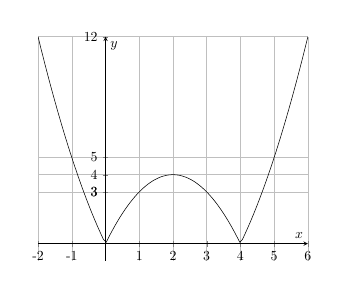
\begin{tikzpicture}[scale=0.5]
\begin{axis}[
    axis lines = middle,
    grid=major,
    legend pos={south west},
    xlabel = {$x$},
    %xlabel style={below right},
    ylabel = {$y$},
    ymin=-1,
    ymax=12,
    xmin=-2,
    xmax=6,
    xtick={-2,-1,1,2,3,4,5,6},
    xticklabels={-2,-1,1,2,3,4,5,6},
    ytick={5,3,12,3,4},
    yticklabels={5,3,12,3,4},
                  ]
	\addplot[domain=-2:6, samples=100, color=black] {abs(x*x-4*x)};
   % \addplot[domain=-3:3, samples=100, color=black] {-x};
     %\addlegendentry{$\text{Рис. 1}$};
\end{axis}
\end{tikzpicture}$$
 По графику найдём $a\in\{0\}\cup(4;+\infty).$\\
